\begin{figure*}[t]
\centering
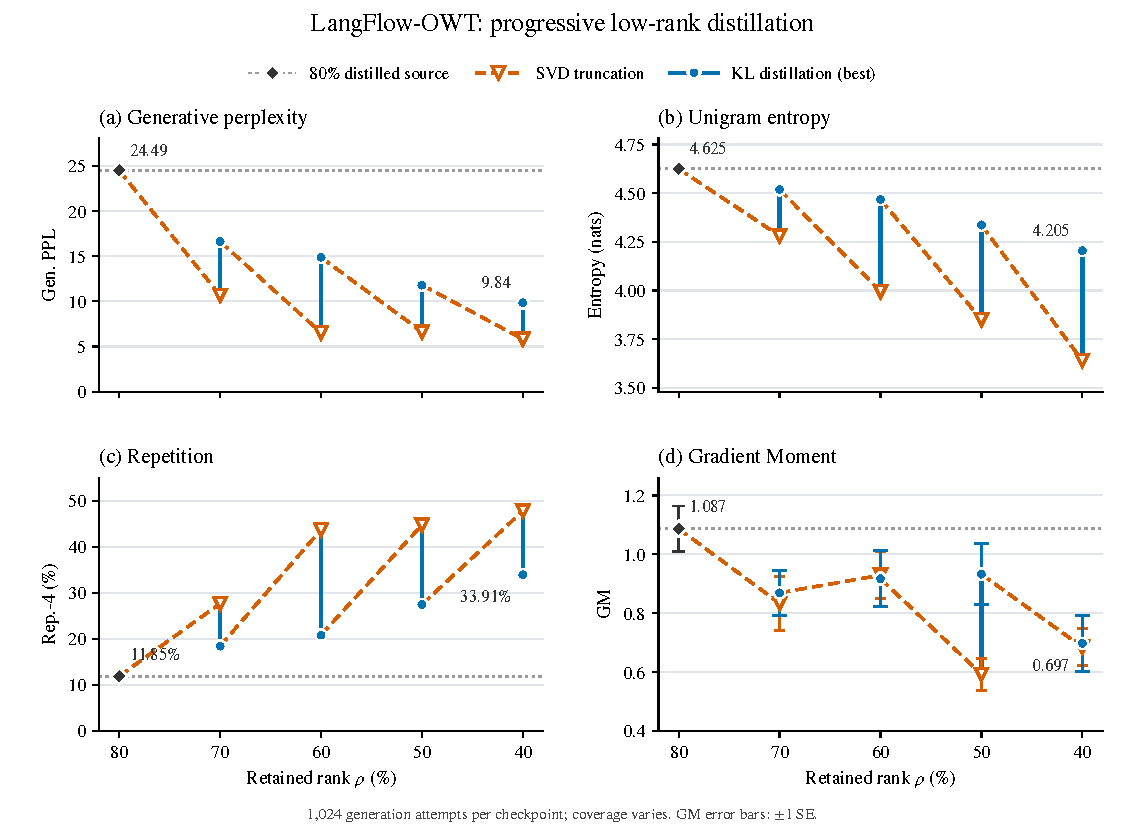
\includegraphics[width=\textwidth]{progressive_080_040.pdf}
\caption{Progressive low-rank distillation from the independently distilled 80\%
student to 40\% rank. Each dashed segment connects the preceding rank's
validation-best student to the next SVD-truncated student. Each solid vertical
segment connects that initialization to the validation-best checkpoint after KL
distillation at the same rank. Gray dotted lines show the re-evaluated 80\%
source values. Distillation partially restores entropy and reduces repetition
after each truncation, while the distilled checkpoints become progressively
more repetitive along the chain. Lower Gen.\ PPL therefore coexists with a loss
of diversity. Each checkpoint attempts 1,024 samples; PPL uses 1,014--1,024
scorable texts, and GM uses 502--512 valid pairs out of 512. GM error bars are
$\pm$ one standard error.}
\label{fig:progressive_low_rank}
\end{figure*}
